\documentclass[conference]{IEEEtran}

\usepackage{cite}
\usepackage{amsmath,amssymb,amsfonts}
\usepackage{algorithmic}
\usepackage{graphicx}
\usepackage{textcomp}
\usepackage[table,xcdraw]{xcolor}
\usepackage{listings}

\lstdefinestyle{pythonstyle}{
    language=Python,
    basicstyle=\ttfamily\small,
    keywordstyle=\color{blue},
    commentstyle=\color{gray},
    stringstyle=\color{teal},
    showstringspaces=false,
    frame=single
}

\lstset{style=pythonstyle}

\def\BibTeX{{\rm B\kern-.05em{\sc i\kern-.025em b}\kern-.08em
    T\kern-.1667em\lower.7ex\hbox{E}\kern-.125emX}}

\begin{document}

\title{Accelerometer and Gyroscope based IoT System for Activity Classification and Monitoring\\
}

\author{\IEEEauthorblockN{Séamus Knightly}
\IEEEauthorblockA{\textit{1MECE1} \\
\textit{University Of Galway}\\
Galway, Ireland\\
s.knightly1@universityofgalway.ie}
\and
\IEEEauthorblockN{Seán Kelly}
\IEEEauthorblockA{\textit{1MECE1} \\
\textit{University Of Galway}\\
Galway, Ireland \\
s.kelly178@universityofgalway.ie}
}

\maketitle

\begin{abstract}
This document is a model and instructions for \LaTeX.
YOLKS YOLKS YOLKS YOLKS YOLKS YOLKS YOLKS YOLKS YOLKS YOLKS YOLKS YOLKS YOLKS YOLKS YOLKS YOLKS YOLKS YOLKS YOLKS YOLKS YOLKS 
\end{abstract}

\begin{IEEEkeywords}
IoT, Remote Patient Monitoring, Accelerometer, Gyroscope, Classification, Assisted Living
\end{IEEEkeywords}

\section{Introduction}


\subsection{Problem Statement}

\subsubsection{Current Situation}
Real-time monitoring of human activity has valuable applications in healthcare, helping to improve patient care, reduce the workload on healthcare staff, and lower costs while enhancing quality of life \cite{b1}. The INMO has stated that the nursing shortage which began in 2007 continues to worsen into 2025\cite{inmo}. This shortage continues to affect rehabilitation facilities, senior living facilities, and other areas where patient movement is key to recovery and continued health.

\subsubsection{Need for IoT System}
Despite this potential, many current monitoring solutions remain limited. Systems such as pendant alarms, deployed through initiatives like the Seniors Alert Scheme, require manual activation by the user in the event of a fall \cite{b2}. This dependency on user input makes them less reliable in emergency situations. Automatic fall detection systems still face challenges with false alarms and missed detections. One study reported that an accelerometer based prototype detected only 80\% of real world falls, with false alarms occurring approximately once every 40 hours of use \cite{b3}. These technological limitations are compounded by staff shortages in the health and social care sector, which place additional strain on staff morale and reduce care quality \cite{b4}. These factors show that there is a need for reliable IoT based solutions that can provide continuous, accurate, and scalable monitoring, which can serve as the foundation for a real-time fall detection monitoring system. This project aims to build a reliable system which fulfils a real-world need, and provides a foundation for future work in this area.

\subsubsection{Aim and Objectives}\label{AO}
The aim of this project is to design and implement an IoT system for activity classification and monitoring using inertial sensors and machine learning. The objectives are to:
\begin{itemize}
	\item Acquire accelerometer and gyroscope data from an IoT device
	\item Transmit sensor data in real time to an IoT gateway
	\item Perform preprocessing at the gateway, including filtering, windowing, and feature extraction
	\item Push the data to a Cloud-based Machine Learning and Data Analytics platform for classification and storage
	\item Implement monitoring of the time-series data with configurable alarms based on healthcare needs
\end{itemize}

\section{System Design}

\subsection{Design Requirements}
There are several key requirements which must be considered when designing wearable IoT devices:
\begin{itemize}
	\item Long operational period / battery life
	\item Medium-range communication - 10-30 meters including walls
	\item Reliable data transmission
	\item Accurate sensing - for activity classification, accurate motion sensing
	\item Comfort - wearables need to be small and lightweight
\end{itemize}

The device must be able to run for at least 24 hours, ideally much longer, between charges to avoid frequent patient disturbance and unnecessary additional work for healthcare workers. The device ideally needs to be able to communicate at medium-range including at least one wall in a hospital or senior living environment if it is to be an effective activity tracker. With the goal of the project being real-time classification and alerting, the data stream needs to be consistent and reliable, not reconnecting frequently or dropping packets. Additionally, the sensors employed for motion sensing, mainly accelerometers and gyroscopes, must be precise enough to allow the classifier to distinguish between different activities, however this is less of a concern as smartphones have had this technology for over a decade. The component selections outlined in Section~\ref{components} aim to fulfil or exceed all of these requirements where possible, whilst also outlining a suitable prototyping platform for the device.

\subsection{Block diagram of the IoT system}
The overall architecture of the IoT system is illustrated in Fig.~\ref{fig:block_diagram}. The future expansion of the project is represented by the blocks with dotted outlines.

\begin{figure}[h]
	\centering
	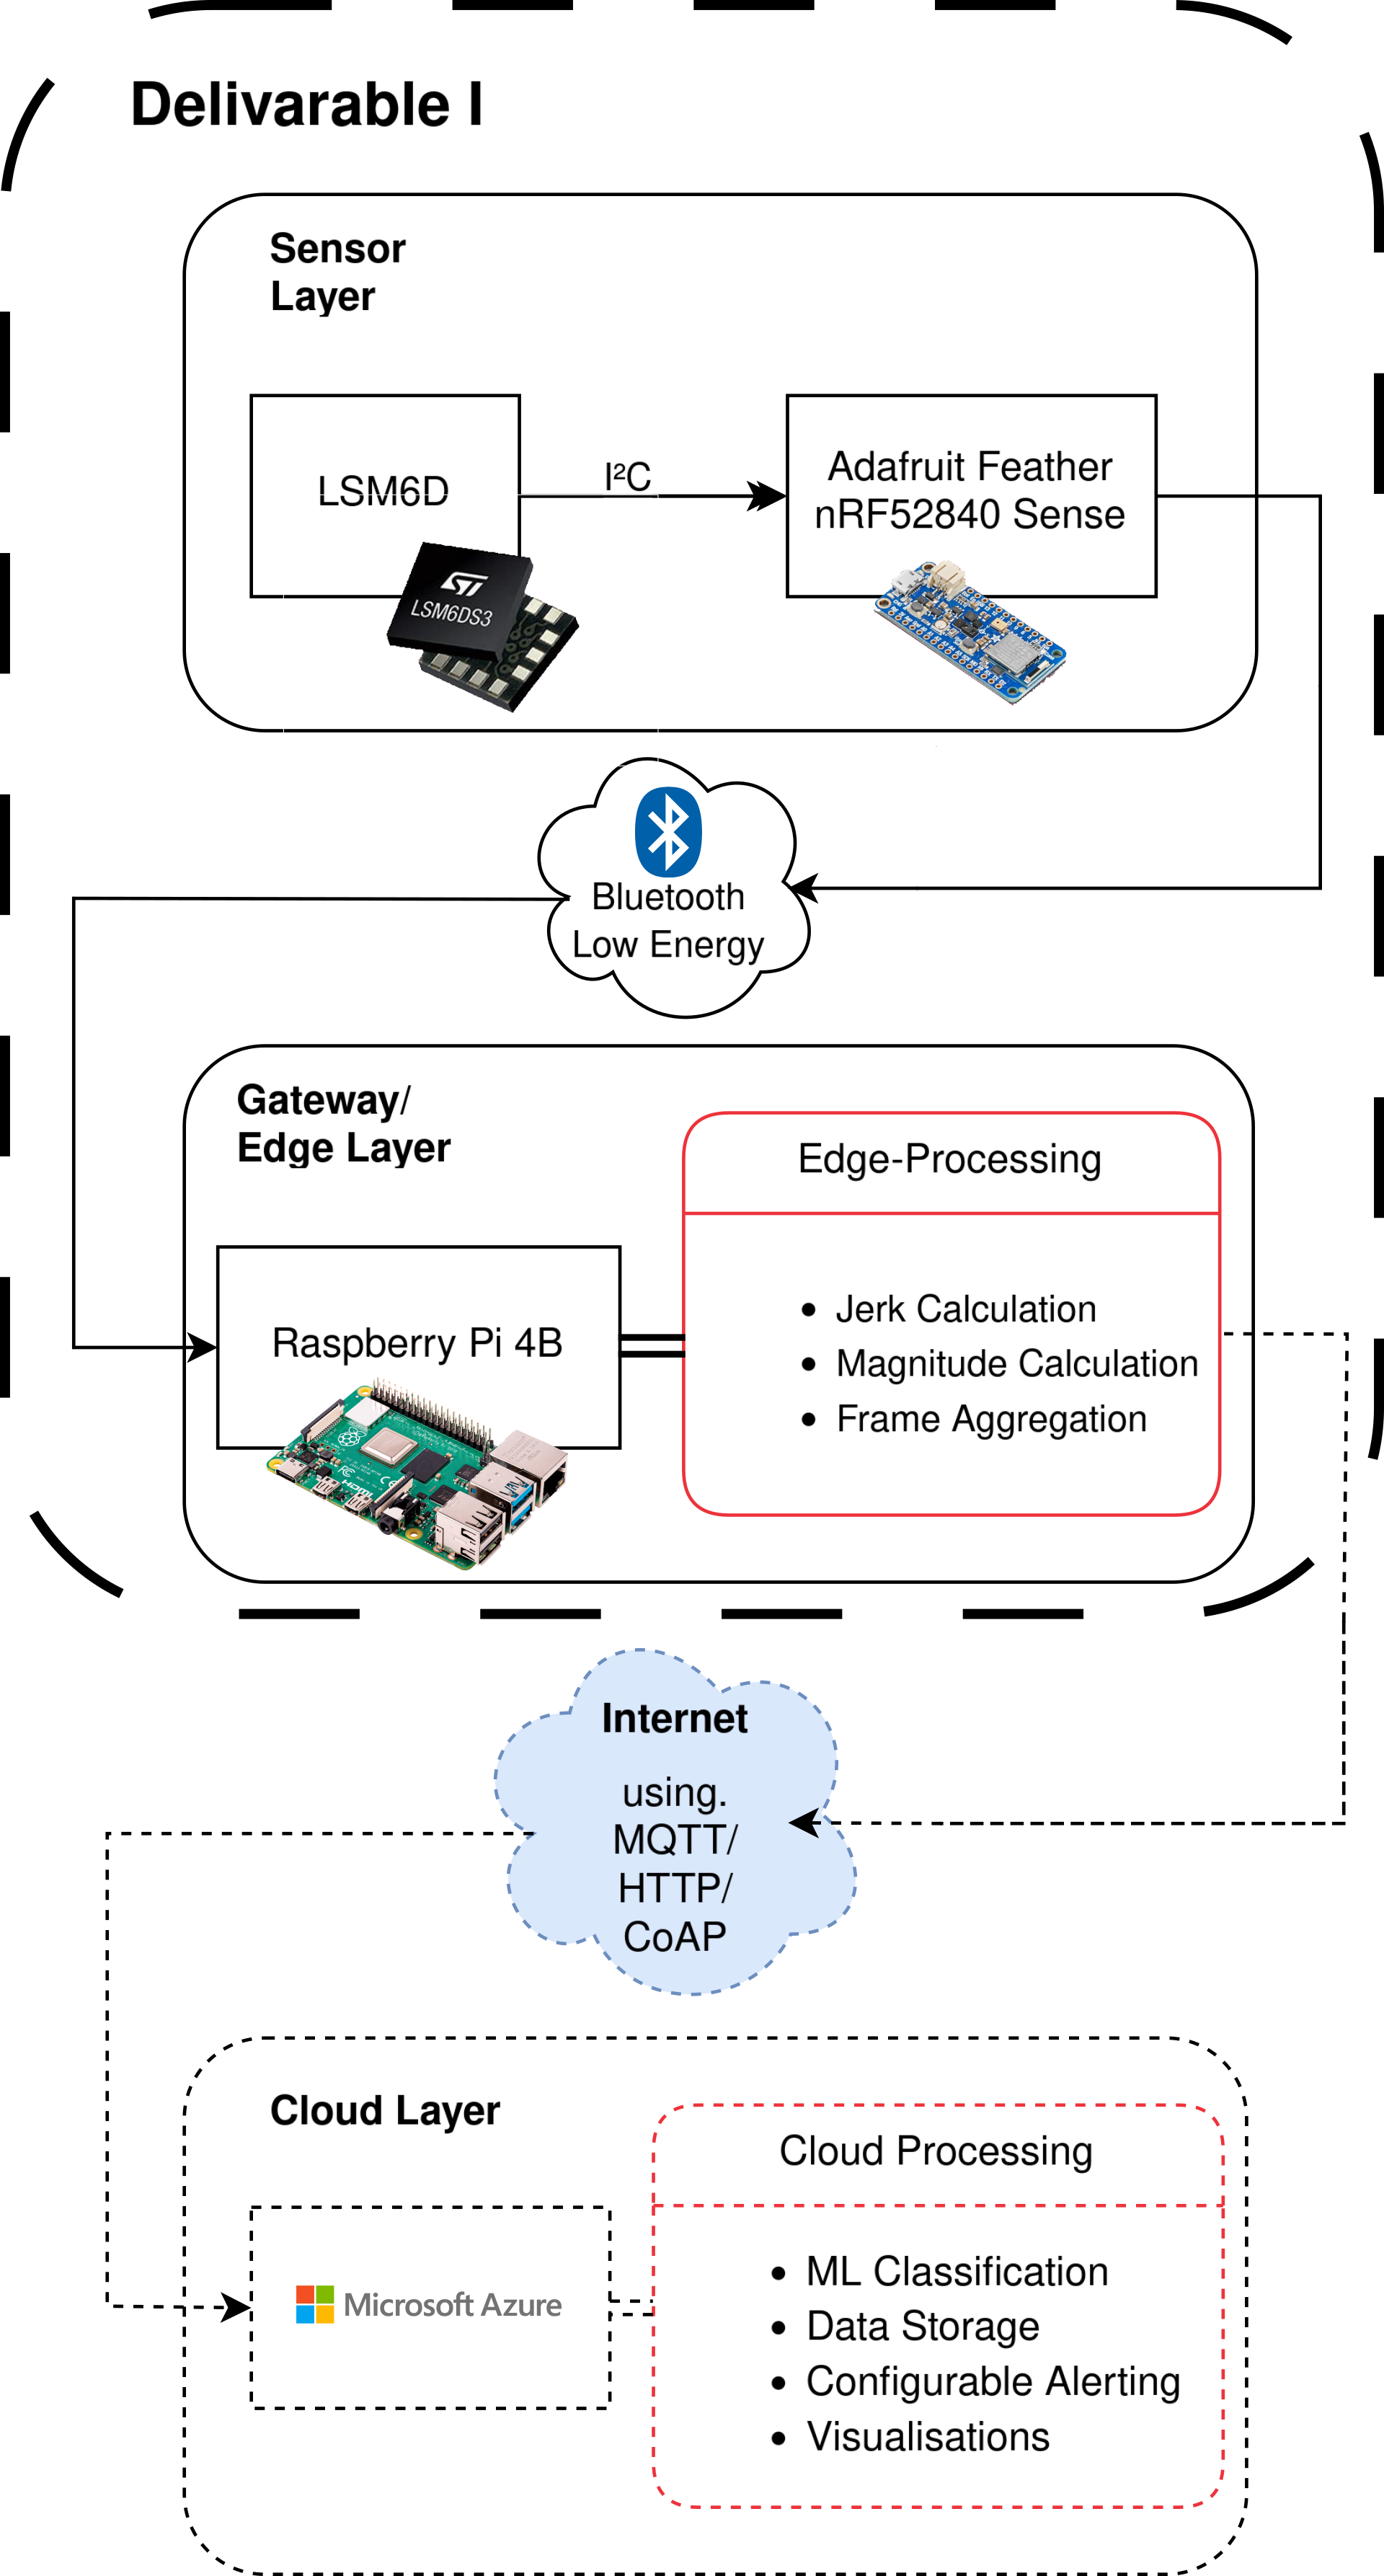
\includegraphics[width=0.9\columnwidth]{media/basic_architecture_overview.png}
	\caption{Block diagram of the IoT system, showing the layered design from sensing to future cloud integration.}
	\label{fig:block_diagram}
\end{figure}


\subsection{Simplified IoT architecture}

The system follows a simplified three-layer IoT architecture. The Sensing and Perception Layer is composed of a wearable sensor node, a compact hip-worn device with a 6-axis IMU for motion capture, where 3 axes are provided by the accelerometer and 3 axes are provided by the gyroscope, giving access to detailed movement information. The device also features a microcontroller with an accompanying BLE module, a battery management system module, and a rechargeable battery.

The Gateway / Edge Compute Layer features an IoT Gateway with a BLE module for collecting data from multiple sensor nodes, internet connectivity (by WiFi or Ethernet), and a powerful system-on-chip capable of data filtering, windowing, and feature extraction in real-time for multiple wearable devices. It is intended to be a stationary gateway mounted in a central location where it can capture data from many devices, process it, and push it to a cloud data processing pipeline.

The Application Layer consists of a machine-learning and data analytics pipeline where a machine learning model classifies the current activity using the received data. The classification, time, and received data are saved in a time-series database for long-term storage, allowing healthcare professionals to access historical activity data for their patients, and configure alerting for patients who are idle for too long or who may be over-active during their recovery.

\section{Component Selections}\label{components}

\subsection{Sensing module}
The BMI160 Low-Power 6-Axis IMU\cite{BMI160} combines a 3-axis accelerometer and a 3-axis gyroscope, both supporting $\pm2G$, $\pm4G$, $\pm8G$, and $\pm16G$ modes, configurable over its serial interface. It uses a simple I2C interface and can operate at voltages between 1.7 and 3.6v, consuming only 1mA when both the accelerometer and gyroscope are active at a 100Hz sample rate. It can be configured to operate at lower sample rates and uses just $180\mu A$ when in accelerometer-only mode at 100Hz. It also features intelligent power management and can go into a sleep state during rest, reactivating the gyroscope only when movement is detected, further reducing power consumption. Bosch advertises this device as an ideal choice for wearable IoT devices.

Altogether this sensor meets the ultra-low power requirement, has more than sufficient resolution at 16-bit, provides all essential data for the machine learning pipeline, and is a widely used option in the field.

The BMI270, also from Bosch SensorTec, is the next-generation model of the BMI160, providing more accuracy, self-calibration, and movement recognition, and while some of these features may be useful in this context, it does not justify the increased cost, significant increase in firmware complexity due to its boot-time configuration requirement, and higher power draw.

Similarly, the MPU-6050, a highly well-known IMU in industry, also elicits a 4x higher power consumption than the BMI160 in a larger package - at 3.9 mA, it is still a viable choice, however with the wide availability of the BMI160, it remains the ideal choice.

\subsection{IoT Node}
The Nordic Semiconductor nRF52810 microcontroller\cite{nRF52810} is an ideal choice for powering the wearable IoT node. It features a 32-bit ARM Cortex-M4 processor running a 64 Mhz, and 192kB flash memory with 24kB of RAM. This is more than sufficient for simple data collection, packaging, and transmission. It also features integrated BLE 5.0 meaning an external module is not needed. It consumes a miniscule $2.0\mu A$ at 3.3 volts when idle, and peaks at just 4.6mA when transmitting or receiving data, making it an ideal choice for a low-power wearable IoT device. The chip also supports ANT, and has a 2.4Ghz transceiver which can be used to develop proprietary protocols if needed.

Another option which was considered is the STM32L031 - an excellent low power option which costs slightly less than the nRF52810, however, this microcontroller does not feature an on-board BLE module, thus ultimately raising the price and design complexity by requiring an external communication IC. 

Other platforms like the Espressif ESP32-C3 are used widely in IoT projects, offering Wi-Fi as well as BLE connectivity, more processing power, and cryptography acceleration\cite{b8}, they typically have a much higher power requirement, as much as 130mA while active. Using these in production comes with an increased cost for no benefit and vastly diminishes battery life.

The Adafruit FeatherSense nRF52840\cite{b7} was chosen as a prototyping board for the project. This board provides a microcontroller from the same family as the production microcontroller, and integrates multiple sensors (e.g., accelerometer/gyroscope, magnetometer, microphone, temperature, humidity, and pressure sensors) along with native BLE support. For this project, only the accelerometer and gyroscope were used, as these sensors correspond with the data requirements of the HARTH dataset \cite{b5,b6} powering the activity classifier in the Cloud IoT pipeline.

\subsection{Gateway}
For this project, the Raspberry Pi 4 serves as the IoT gateway. The Pi 4 Model B 4GB RAM variant features a Broadcom BCM2711, a System-on-Chip containing a quad-core ARM Cortex-A72 processor. All Pi 4 Model Bs feature LPDDR4 memory running at 3200Mhz. It features on-board 2.4Ghz and 5.0Ghz WiFi, Gigabit Ethernet, Bluetooth 5.0 and BLE 5.0, and a Micro SD card slot. The device consumes a maximum of 15w under load, and takes up quite a small space. With the amount of processing available on-board, and at a cost of only \$60 USD, the Pi 4 is an ideal choice for communicating with, and handling data from a large volume of IoT nodes. The Pi 4 runs a full Linux environment by default but can easily be customized to run a stripped back Linux distribution designed solely to run IoT Gateway functions. As it uses Linux, it natively supports Python for prototyping and C/C++ for production deployments as standard, with a wide variety of libraries available for BLE communication, MQTT for sending data to the cloud, edge machine learning libraries, and much more.

Additionally, the Raspberry Pi can be accessed remotely and easily serviced by means of re-imaging should anything go wrong, or if remote diagnostics / application support is required.

An industrial IoT gateway device such as a RAD IoT Gateway could run from hundreds to thousands of euro, and is completely overkill for a small-to-medium scale deployment like in a hospital environment or nursing home. Additionally, it comes with vendor lock-in and increased development times due to is proprietary nature.

\subsection{Communication}
Bluetooth Low Energy 5.0 (BLE 5) was selected for communicating between the IoT Device and the Gateway. The nRF52810 contains an integrated BLE 5 communication module, with a transmit power of up to 4 dBm. With this power, 10-30m range including obstacles can easily be done, at data rates of up to 2 Mbps if necessary. Additionally, BLE is designed for many-to-one communication, making it easy to connect many devices to the Raspberry Pi 4 IoT Gateway.

Other options considered were Zigbee, which is a very low power mesh-networking solution, however it requires a separate network coordinator IC not available on the nRF52810 or the Raspberry Pi. Additionally, it features much lower data rates, and a mesh network is not needed for a deployment of the proposed size.

WiFi HaLow was also considered initially due to its long range and configurable data rates, however it also requires external hardware and has a much higher power requirement than BLE 5, making it a less than ideal choice for a wearable device.

The Bluetooth Low Energy protocol is also natively supported by the FeatherSense nRF52840 board. The initial implementation of sensor data communication used BLE UART with Concise Binary Object Representation (CBOR) encoding - ``The Concise Binary Object Representation (CBOR) is a data format whose design goals include the possibility of extremely small code size, fairly small message size, and extensibility without the need for version negotiation.''\cite{cbor}. Ulimately, the UART was too slow to meet the 50~Hz sampling target, and the system was reimplemented using BLE GATT at a data rate of 52 packets per second, where fixed length packets of six floating point values were used. This allowed stable data transmission of at least 50 samples per second for each each of the 6 axes of the IMU.

\subsection{Power}

For power, a pair of AA-sized rechargeable Lithium Iron Phosphate (LiFePO4) batteries, combined with a Nordic Semiconductor nPM1300 Power Management IC, which brings power regulation for the microcontroller, battery level gauging, a system-level power watchdog, and battery charge management compatible with LiFePO4 and supporting USB-C as standard.

The Lithium Iron Phosphate Battery in AA size is an ideal choice for the amount of space available, and is much safer than options such as Lithium Ion or Lithium Polymer batteries which can fail catastrophically if over-discharged, improperly recharged, or pierced. Each AA-sized LiFePo battery has a 600 mAh capacity, together allowing the device to run for days at a time. They are lightweight, weighing just 18 grams each, and most importantly, can support over 2000 charge cycles when using an 80\% Depth of Discharge, which can be done using the nPM1300. 

Other alternatives considered were Lithium Ion and Lithium Polymer batteries, but both solutions are less stable and have a lower energy density than LiFePo4 batteries. For battery management and voltage regulation, the MCP73831 charging IC was considered for many of the same reasons as the nPM1300 - it supports USB-C, a 3.2v nominal battery voltage, automatic charge termination, and status indicators. This, in combination with the TPS62840 buck converter for voltage regulation, which supports converting 6.4v to 3.3v at a 90\% efficiency at the proposed loads, was the original power system designed for the device. Given that both devices could be combined into a single chip with a system-level power watchdog and battery level gauge if the nPM1300 was used, this led to their removal from the design.

For prototyping, the FeatherSense board was powered via USB using a battery pack, which allowed for quick and easy testing after programming the device via USB. 

\section{Prototype Design Plan}

\subsection{Subsystems}
The prototype will be structured into four main subsystems: 
\begin{itemize}
	\item \textbf{Sensing:} Inertial data acquisition from the FeatherSense accelerometer and gyroscope. 
	\item \textbf{Communication:} Wireless transmission via BLE, using GATT as the chosen protocol. 
	\item \textbf{Edge Processing:} Real-time data handling and basic feature extraction on the Raspberry Pi 4. 
	\item \textbf{Visualisation:} Plotting of data streams to confirm correct reception and interpretation. 
\end{itemize}
This breakdown will ensure that each component of the system can be developed and validated independently before integration. 

\subsection{Integration Plan}
The system will be developed incrementally. The sensor subsystem will first be validated by confirming raw inertial readings on the FeatherSense. Next, BLE transmission will be tested in isolation before final integration. This will be followed by configuring the gateway to receive and interpret data packets, after which the noise filtering, data windowing, and feature extraction will be added. Each of these features are tested in isolation with pre-captured data, then integrated into the full application to test its functionality with real-time data. 

\subsection{Verification Plan}
Verification activities will be designed to ensure that the prototype meets Deliverable~I requirements. The main checks will include:
\begin{itemize}
	\item Confirming that BLE transmission achieves the target 50~Hz sampling rate
	\item Ensuring data packets are correctly structured and fully decoded at the gateway
	\item Validating that received sensor values fall within expected physical ranges (e.g., acceleration values near $\pm 9.8~\text{m/s}^2$ for gravity)
\end{itemize}

\section{Implementation}
\subsection{Feathersense Node Setup}
For prototyping and software development, the sensor node was implemented using the Adafruit FeatherSense nRF52840 board. The LSM6DS3 IMU was configured to sample at 50Hz, in line with the publicly available HARTH dataset. Sensor readings (acceleration in m/s\textsuperscript{2} and angular velocity in deg/s) were acquired in real time through the Adafruit CircuitPython libraries. 

\subsection{Communication Performance}
An initial implementation used the Nordic UART Service over BLE, with payloads encoded in CBOR format. This implementation was functional, but very inefficient. The structured CBOR packets were relatively large, so the transmission was slower and there was an increased coding and decoding overhead on both device and gateway. As a result, the effective sampling rate was limited to approximately 11~Hz, and partial reads often caused incomplete or dropped data. The performance was too poor due to the low data rate of the UART, to be considered as an option.

To address the issues found with the UART method, the system was reimplemented using a custom GATT service with two vendor-defined UUIDs (one for the service and one for the sensor characteristic). Instead of transmitting dictionary structures, the new approach packed six 32 bit floating point values (ax, ay, az, gx, gy, gz) into a fixed length 24 byte payload. This enabled stable streaming at the target rate of 50~Hz without the packet corruption or decoding delays observed previously.

\section{Implementation of Gateway Device}
\subsection{Data collection on Raspberry Pi}\label{data_collection}
The implementation of the Bluetooth Low Energy connection and data retrieval via GATT was implemented using the Bleak Python library, which provides a Bluetooth Scanner and Bluetooth Client. Together, these allow you to first discover all Bluetooth devices advertising in the vicinity, find an address corresponding to an advertised name, and then spawn a Bluetooth Client targetting that address. Bleak also provides a callback service which can trigger a notification handler when a notification arrives from a specific characteristic of a service. This was used to subscribe to the characteristic sending sensor data to the gateway at 50Hz.

The Gateway application first connects to the IoT node, then sets up the characteristic subscription. This triggers a calibration process which calculates the zero values for each axis by taking 50 samples and averaging them, then storing them as fixed offsets - this results in all readings being zero when the device is perfectly still in its default orientation. A deadzone of 0.1m/s and 0.1 rad/s removes some of the jitter from the signal without taking away resolution of fine motor control.

Finally, the gateway takes a 128 sample window with a 50\% overlap, which brings the data into the same format as the dataset, making it suitable for further processing to find the sample window mean, fourier transform, and other features.

For convenience, the program also contains an asynchronous plotting routine using MatPlotLib to plot the data in real-time.

\subsection{Streaming Visualisation}
The graphs shown in Figure \ref{fig:basic_data} were generated by the code outlined in Section  \ref{data_collection}. The exact code used on the IoT Device can be found in Appendix \ref{iot_firmware}.

\begin{figure}[h]
	\centering
	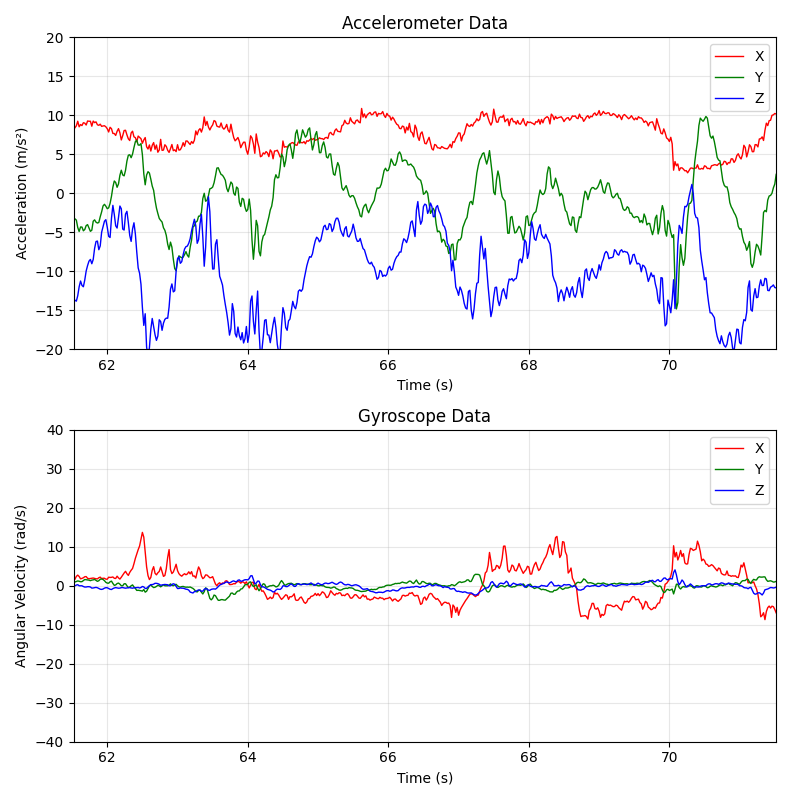
\includegraphics[width=0.9\columnwidth]{media/Figure_1.png}
	\caption{A rendering of a sample window containing filtered gyrometer and accelerometer data}
	\label{fig:basic_data}
\end{figure}

\section{Edge/Fog Processing}
\subsection{Feature Extraction on Raspberry Pi}\label{feature_extraction}
Jerk calculation (derivative of acceleration).

Magnitude of accel/gyro.

Other features relevant for ML (you can mention RMS, variance, etc. if planned).

Show small plots of raw vs processed features.

\subsection{Feature Extraction Visualisation}
The graphs shown in Figure \ref{fig:extracted_data} were generated by the code outlined in Section  \ref{feature_extraction}. The exact code used on the Gateway Device can be found in Appendix \ref{gateway_firmware}.

\begin{figure}[h]
	\centering
	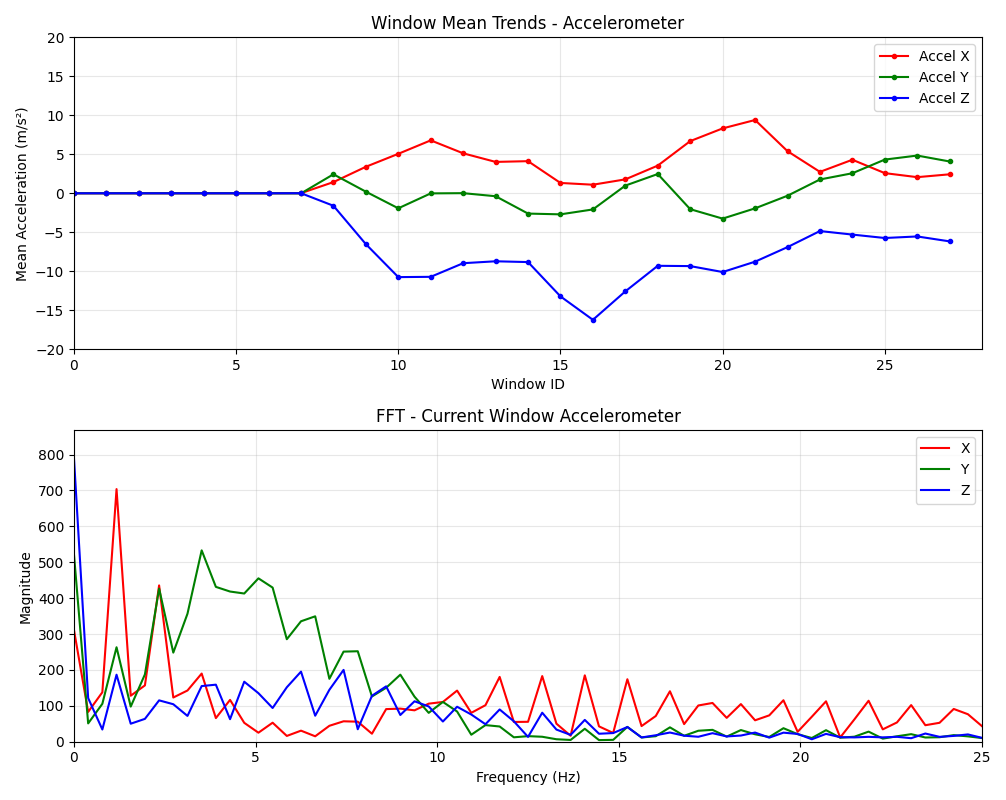
\includegraphics[width=0.9\columnwidth]{media/Figure_2.png}
	\caption{A rendering of the mean accelerations for the previous 50 windows and the FFT of the current data window}
	\label{fig:extracted_data}
\end{figure}

\section{Discussion \& Conclusion}
Summary: successful acquisition, transmission, preprocessing.

Limitations: still simulated/early prototype, real-world testing needed.

Next steps (for Deliverable II): deploy ML in cloud, integrate with Power BI.

\bibliographystyle{IEEEtran}
\bibliography{references}

\onecolumn

\appendices
\section{IoT Device Firmware}\label{iot_firmware}
\begin{lstlisting}[language=Python]
import struct
import time
import board
import asyncio

from adafruit_ble import BLERadio
from adafruit_lsm6ds import Rate, AccelRange, GyroRange
from adafruit_ble.advertising.standard import ProvideServicesAdvertisement
from adafruit_ble.services import Service
from adafruit_ble.characteristics import Characteristic
from adafruit_ble.uuid import VendorUUID

# Custom BLE Service
class SensorService(Service):
    uuid = VendorUUID("12345678-1234-5678-1234-56789abcdef0")
    sensor_data = Characteristic(
        uuid=VendorUUID("12345678-1234-5678-1234-56789abcdef1"),
        properties=Characteristic.NOTIFY,
        max_length=24  # 6 floats * 4 bytes each
    )

i2c = board.I2C()

try:
    from adafruit_lsm6ds.lsm6ds33 import LSM6DS33 as LSM6DS
    lsm6ds = LSM6DS(i2c)
except RuntimeError:
    from adafruit_lsm6ds.lsm6ds3 import LSM6DS3 as LSM6DS
    lsm6ds = LSM6DS(i2c)

lsm6ds.accelerometer_data_rate = Rate.RATE_3_33K_HZ
lsm6ds.gyro_data_rate = Rate.RATE_3_33K_HZ

lsm6ds.accelerometer_range = AccelRange.RANGE_8G
lsm6ds.gyro_range = GyroRange.RANGE_2000_DPS

ble = BLERadio()
ble.name = "Old Person Life Invader"
sensor_service = SensorService()
advertisement = ProvideServicesAdvertisement(sensor_service)

target_dt = 1.0 / 50.0  # 50 Hz

while True:
    print(f"BLE name: {ble.name}")
    print(f"AccelRange set to: {AccelRange.string[lsm6ds.accelerometer_range]}")
    print(f"GyroRange set to: {GyroRange.string[lsm6ds.gyro_range]}")
    ble.start_advertising(advertisement)

    while ble.connected:
        t0 = time.monotonic()

        # Read accel + gyro
        accel = lsm6ds.acceleration   # (x,y,z)
        gyro  = lsm6ds.gyro           # (x,y,z)

        # Pack all 6 floats: ax, ay, az, gx, gy, gz
        payload = struct.pack("<ffffff",
                              accel[0], accel[1], accel[2],
                              gyro[0],  gyro[1],  gyro[2])

        try:
            sensor_service.sensor_data = payload
        except Exception:
            pass

        # maintain ~50 Hz
        dt = time.monotonic() - t0
        if dt < target_dt:
            time.sleep(target_dt - dt)
\end{lstlisting}

\section{IoT Gateway Application}\label{gateway_firmware}
\begin{lstlisting}[language=Python]
import asyncio
import struct
import io
import logging
from bleak import BleakScanner, BleakClient
from collections import deque
import statistics
import matplotlib.pyplot as plt
import matplotlib.animation as animation
from threading import Thread, Lock
import numpy as np

SERVICE_UUID = "12345678-1234-5678-1234-56789abcdef0"
CHAR_UUID    = "12345678-1234-5678-1234-56789abcdef1"

# Calibration settings
CALIBRATION_SAMPLES = 50  # Number of samples to average for calibration
NOISE_THRESHOLD = 0.1     # Values below this are considered noise (m/s^2 or dps)

# Windowing settings
WINDOW_SIZE = 128         # 2.56 seconds at 50 Hz
WINDOW_STEP = 64          # 50% overlap (step by half the window size)
SAMPLE_RATE = 50          # Hz

# Configure logging
logger = logging.getLogger()
logger.setLevel(logging.INFO)

# Remove any existing handlers
for handler in logger.handlers[:]:
    logger.removeHandler(handler)

# Create a custom formatter with no prefix
csv_formatter = logging.Formatter('%(message)s')

# Create file handler that dumps logged data to CSV
file_handler = logging.FileHandler('data.csv', mode='w')
file_handler.setFormatter(csv_formatter)
logger.addHandler(file_handler)

# Create console handler that outputs normal logs to console
console_handler = logging.StreamHandler()
logger.addHandler(console_handler)

class PlotData:
    """Thread-safe container for plot data"""
    def __init__(self):
        self.lock = Lock()
        
        # Current window data (only the latest window)
        self.current_window = None
        self.window_timestamps = None
        
        # Historical window means for trending
        self.window_means_ax = deque(maxlen=50)  # Keep last 50 windows
        self.window_means_ay = deque(maxlen=50)
        self.window_means_az = deque(maxlen=50)
        self.window_means_gx = deque(maxlen=50)
        self.window_means_gy = deque(maxlen=50)
        self.window_means_gz = deque(maxlen=50)
        self.window_ids = deque(maxlen=50)
        
        self.window_count = 0
    
    def update_window(self, window_data):
        """Update with a new complete window"""
        with self.lock:
            # Convert window to numpy array
            window_array = np.array(window_data)
            self.current_window = window_array
            self.window_timestamps = np.arange(len(window_data)) / SAMPLE_RATE
            
            # Calculate means for this window
            means = np.mean(window_array, axis=0)
            self.window_means_ax.append(means[0])
            self.window_means_ay.append(means[1])
            self.window_means_az.append(means[2])
            self.window_means_gx.append(means[3])
            self.window_means_gy.append(means[4])
            self.window_means_gz.append(means[5])
            
            self.window_ids.append(self.window_count)
            self.window_count += 1
    
    def get_current_window(self):
        """Get current window data (thread-safe)"""
        with self.lock:
            if self.current_window is None:
                return None, None
            return self.current_window.copy(), self.window_timestamps.copy()
    
    def get_window_means(self):
        """Get historical window means (thread-safe)"""
        with self.lock:
            if len(self.window_ids) == 0:
                return None
            return {
                'ids': list(self.window_ids),
                'ax': list(self.window_means_ax),
                'ay': list(self.window_means_ay),
                'az': list(self.window_means_az),
                'gx': list(self.window_means_gx),
                'gy': list(self.window_means_gy),
                'gz': list(self.window_means_gz)
            }

# Global plot data
plot_data = PlotData()

class SensorProcessor:
    def __init__(self):
        # Calibration offsets
        self.ax_offset = 0.0
        self.ay_offset = 0.0
        self.az_offset = 0.0
        self.gx_offset = 0.0
        self.gy_offset = 0.0
        self.gz_offset = 0.0
        
        # Calibration data collection
        self.calibration_data = []
        self.is_calibrated = False
        
        # Sliding window buffer
        self.window_buffer = deque(maxlen=WINDOW_SIZE)
        self.samples_since_last_window = 0
        
    def add_calibration_sample(self, ax, ay, az, gx, gy, gz):
        """Collect samples for calibration"""
        self.calibration_data.append((ax, ay, az, gx, gy, gz))
        
        if len(self.calibration_data) >= CALIBRATION_SAMPLES:
            self._compute_offsets()
            return True
        return False
    
    def _compute_offsets(self):
        """Compute average offsets from calibration samples"""
        ax_samples = [s[0] for s in self.calibration_data]
        ay_samples = [s[1] for s in self.calibration_data]
        az_samples = [s[2] for s in self.calibration_data]
        gx_samples = [s[3] for s in self.calibration_data]
        gy_samples = [s[4] for s in self.calibration_data]
        gz_samples = [s[5] for s in self.calibration_data]
        
        self.ax_offset = statistics.mean(ax_samples)
        self.ay_offset = statistics.mean(ay_samples)
        self.az_offset = statistics.mean(az_samples)
        self.gx_offset = statistics.mean(gx_samples)
        self.gy_offset = statistics.mean(gy_samples)
        self.gz_offset = statistics.mean(gz_samples)
        
        self.is_calibrated = True
        logger.info(f"Calibration complete: ax={self.ax_offset:.3f}, ay={self.ay_offset:.3f}, "
                   f"az={self.az_offset:.3f}, gx={self.gx_offset:.3f}, gy={self.gy_offset:.3f}, "
                   f"gz={self.gz_offset:.3f}")
    
    def apply_noise_filter(self, value):
        """Apply dead-zone filter to remove small noise"""
        return 0.0 if abs(value) < NOISE_THRESHOLD else value
    
    def process(self, ax, ay, az, gx, gy, gz):
        """Apply calibration and noise filtering"""
        # Apply offsets
        ax_cal = ax - self.ax_offset
        ay_cal = ay - self.ay_offset
        az_cal = az - self.az_offset
        gx_cal = gx - self.gx_offset
        gy_cal = gy - self.gy_offset
        gz_cal = gz - self.gz_offset
        
        # Apply noise filter
        ax_filtered = self.apply_noise_filter(ax_cal)
        ay_filtered = self.apply_noise_filter(ay_cal)
        az_filtered = self.apply_noise_filter(az_cal)
        gx_filtered = self.apply_noise_filter(gx_cal)
        gy_filtered = self.apply_noise_filter(gy_cal)
        gz_filtered = self.apply_noise_filter(gz_cal)
        
        return ax_filtered, ay_filtered, az_filtered, gx_filtered, gy_filtered, gz_filtered
    
    def add_to_window(self, ax, ay, az, gx, gy, gz):
        """Add sample to sliding window and return window when ready"""
        self.window_buffer.append((ax, ay, az, gx, gy, gz))
        self.samples_since_last_window += 1
        
        # Check if we have a full window and have stepped far enough
        if len(self.window_buffer) == WINDOW_SIZE and self.samples_since_last_window >= WINDOW_STEP:
            self.samples_since_last_window = 0
            # Return a copy of the current window
            return list(self.window_buffer)
        
        return None

# Global sensor processor
sensor_processor = SensorProcessor()

def handle_notification(_, data: bytearray):
    try:
        ax, ay, az, gx, gy, gz = struct.unpack("<ffffff", data)
        
        # Calibration phase
        if not sensor_processor.is_calibrated:
            calibrated = sensor_processor.add_calibration_sample(ax, ay, az, gx, gy, gz)
            if calibrated:
                logger.info("window_id,sample_id,acceleration_x,acceleration_y,acceleration_z,gyro_x,gyro_y,gyro_z")
            return
        
        # Process data with calibration and filtering
        ax_f, ay_f, az_f, gx_f, gy_f, gz_f = sensor_processor.process(ax, ay, az, gx, gy, gz)
        
        # Add to sliding window
        window = sensor_processor.add_to_window(ax_f, ay_f, az_f, gx_f, gy_f, gz_f)
        
        # If we have a complete window, log it and update plot
        if window is not None:
            window_id = (len(sensor_processor.window_buffer) - WINDOW_SIZE) // WINDOW_STEP + 1
            for sample_id, (ax, ay, az, gx, gy, gz) in enumerate(window):
                logger.info(f"{window_id},{sample_id},{ax:.1f},{ay:.1f},{az:.1f},{gx:.1f},{gy:.1f},{gz:.1f}")
            
            # Update plot data with new window
            plot_data.update_window(window)
    except Exception as e:
        logger.error(f"Decode error: {e}")

def setup_plot_window1():
    """Setup first plotting window - current window raw data"""
    fig, (ax1, ax2) = plt.subplots(2, 1, figsize=(10, 8))
    fig.canvas.manager.set_window_title('Window 1: Current Window Data')
    
    # Accelerometer plot
    line_ax, = ax1.plot([], [], 'r-', label='X', linewidth=1.5)
    line_ay, = ax1.plot([], [], 'g-', label='Y', linewidth=1.5)
    line_az, = ax1.plot([], [], 'b-', label='Z', linewidth=1.5)
    ax1.set_xlim(0, WINDOW_SIZE / SAMPLE_RATE)
    ax1.set_ylim(-20, 20)
    ax1.set_xlabel('Time (s)')
    ax1.set_ylabel('Acceleration (m/s^2)')
    ax1.set_title('Current Window - Accelerometer Data')
    ax1.legend(loc='upper right')
    ax1.grid(True, alpha=0.3)
    
    # Gyroscope plot
    line_gx, = ax2.plot([], [], 'r-', label='X', linewidth=1.5)
    line_gy, = ax2.plot([], [], 'g-', label='Y', linewidth=1.5)
    line_gz, = ax2.plot([], [], 'b-', label='Z', linewidth=1.5)
    ax2.set_xlim(0, WINDOW_SIZE / SAMPLE_RATE)
    ax2.set_ylim(-40, 40)
    ax2.set_xlabel('Time (s)')
    ax2.set_ylabel('Angular Velocity (rad/s)')
    ax2.set_title('Current Window - Gyroscope Data')
    ax2.legend(loc='upper right')
    ax2.grid(True, alpha=0.3)
    
    plt.tight_layout()
    
    lines = {
        'ax': line_ax, 'ay': line_ay, 'az': line_az,
        'gx': line_gx, 'gy': line_gy, 'gz': line_gz
    }
    
    return fig, ax1, ax2, lines

def setup_plot_window2():
    """Setup second plotting window - means and FFT"""
    fig, (ax1, ax2) = plt.subplots(2, 1, figsize=(10, 8))
    fig.canvas.manager.set_window_title('Window 2: Trends and FFT Analysis')
    
    # Window means plot
    line_ax, = ax1.plot([], [], 'r-', label='Accel X', linewidth=1.5, marker='o', markersize=3)
    line_ay, = ax1.plot([], [], 'g-', label='Accel Y', linewidth=1.5, marker='o', markersize=3)
    line_az, = ax1.plot([], [], 'b-', label='Accel Z', linewidth=1.5, marker='o', markersize=3)
    ax1.set_xlabel('Window ID')
    ax1.set_ylabel('Mean Acceleration (m/s^2)')
    ax1.set_ylim(-20, 20)
    ax1.set_title('Window Mean Trends - Accelerometer')
    ax1.legend(loc='upper right')
    ax1.grid(True, alpha=0.3)
    
    # FFT plot
    line_fft_x, = ax2.plot([], [], 'r-', label='X', linewidth=1.5)
    line_fft_y, = ax2.plot([], [], 'g-', label='Y', linewidth=1.5)
    line_fft_z, = ax2.plot([], [], 'b-', label='Z', linewidth=1.5)
    ax2.set_xlim(0, SAMPLE_RATE / 2)  # Nyquist frequency
    ax2.set_ylim(0, 10)
    ax2.set_xlabel('Frequency (Hz)')
    ax2.set_ylabel('Magnitude')
    ax2.set_title('FFT - Current Window Accelerometer')
    ax2.legend(loc='upper right')
    ax2.grid(True, alpha=0.3)
    
    plt.tight_layout()
    
    lines = {
        'ax': line_ax, 'ay': line_ay, 'az': line_az,
        'fft_x': line_fft_x, 'fft_y': line_fft_y, 'fft_z': line_fft_z
    }
    
    return fig, ax1, ax2, lines

def animate_window1(frame, ax1, ax2, lines):
    """Animation function for window 1 - current window data"""
    window_data, timestamps = plot_data.get_current_window()
    
    if window_data is None:
        return lines.values()
    
    # Update accelerometer lines
    lines['ax'].set_data(timestamps, window_data[:, 0])
    lines['ay'].set_data(timestamps, window_data[:, 1])
    lines['az'].set_data(timestamps, window_data[:, 2])
    
    # Update gyroscope lines
    lines['gx'].set_data(timestamps, window_data[:, 3])
    lines['gy'].set_data(timestamps, window_data[:, 4])
    lines['gz'].set_data(timestamps, window_data[:, 5])
    
    return lines.values()

def animate_window2(frame, ax1, ax2, lines):
    """Animation function for window 2 - means and FFT"""
    # Update window means
    means_data = plot_data.get_window_means()
    
    if means_data is not None:
        lines['ax'].set_data(means_data['ids'], means_data['ax'])
        lines['ay'].set_data(means_data['ids'], means_data['ay'])
        lines['az'].set_data(means_data['ids'], means_data['az'])
        
        # Auto-adjust x-axis for means
        if len(means_data['ids']) > 0:
            ax1.set_xlim(means_data['ids'][0], means_data['ids'][-1] + 1)
    
    # Update FFT
    window_data, _ = plot_data.get_current_window()
    
    if window_data is not None:
        # Compute FFT for each accelerometer axis
        fft_x = np.fft.rfft(window_data[:, 0])
        fft_y = np.fft.rfft(window_data[:, 1])
        fft_z = np.fft.rfft(window_data[:, 2])
        
        # Get frequency bins
        freqs = np.fft.rfftfreq(len(window_data), 1/SAMPLE_RATE)
        
        # Compute magnitudes
        mag_x = np.abs(fft_x)
        mag_y = np.abs(fft_y)
        mag_z = np.abs(fft_z)
        
        # Update FFT lines
        lines['fft_x'].set_data(freqs, mag_x)
        lines['fft_y'].set_data(freqs, mag_y)
        lines['fft_z'].set_data(freqs, mag_z)
        
        # Auto-adjust y-axis for FFT
        max_mag = max(np.max(mag_x), np.max(mag_y), np.max(mag_z))
        ax2.set_ylim(0, max_mag * 1.1)
    
    return lines.values()

def start_plots():
    """Start both matplotlib windows in the main thread"""
    # Setup window 1
    fig1, ax1_1, ax2_1, lines1 = setup_plot_window1()
    ani1 = animation.FuncAnimation(
        fig1, animate_window1, 
        fargs=(ax1_1, ax2_1, lines1),
        interval=100,  # 100ms = 10 FPS
        blit=True,
        cache_frame_data=False
    )
    
    # Setup window 2
    fig2, ax1_2, ax2_2, lines2 = setup_plot_window2()
    ani2 = animation.FuncAnimation(
        fig2, animate_window2, 
        fargs=(ax1_2, ax2_2, lines2),
        interval=100,  # 100ms = 10 FPS
        blit=True,
        cache_frame_data=False
    )
    
    plt.show()

async def main():
    # Start matplotlib in a separate thread
    plot_thread = Thread(target=start_plots, daemon=True)
    plot_thread.start()
    
    logger.info("Scanning for BLE devices...")
    devices = await BleakScanner.discover(timeout=5.0)

    target = None
    for d in devices:
        if d.name and "Old Person Life Invader" in d.name:
            target = d
            break

    if not target:
        logger.error("Peripheral not found!")
        return

    async with BleakClient(target.address) as client:
        logger.info(f"Connected to {target.name}")
        logger.info(f"Calibrating sensors... (collecting {CALIBRATION_SAMPLES} samples)")
        logger.info("Please keep device still during calibration")
        
        await client.start_notify(CHAR_UUID, handle_notification)

        try:
            while True:
                await asyncio.sleep(1.0)
        except KeyboardInterrupt:
            logger.info("Disconnecting...")
        finally:
            await client.stop_notify(CHAR_UUID)

if __name__ == "__main__":
    asyncio.run(main())
\end{lstlisting}

\end{document}